\documentclass[12pt]{article}
\usepackage{color}
\usepackage{cite}
\usepackage{geometry}                % See geometry.pdf to learn the layout options. There are lots.
%\usepackage{pdflscape}        %single page landscape
                                %mode \begin{landscape} \end{landscape}
\geometry{letterpaper}                   % ... or a4paper or a5paper or ... 
%\usepackage[parfill]{parskip}    % Activate to begin paragraphs with an empty line rather than an indent
\usepackage{graphicx}
\usepackage{amssymb}
\usepackage{Sweave}
\newcommand{\etal}{\textit{et al.}}
\usepackage{hyperref}  %\hyperref[label_name]{''link text''}
                       %\hyperlink{label}{anchor caption}
                       %\hypertarget{label}{link caption}
\linespread{1.5}

\title{Arthropod Coocurrence Study}
\author{M.K. Lau}
%\date{}                                           % Activate to display a given date or no date

\begin{document}
\maketitle

\textbf{Tasks}
\begin{itemize}
\item Test for number of senescing leaves correlation with Pb
\item Think about direct versus indirect genetic effects on community
\item Test genotype effect on all species
\item Get genetic distance data (RFLP?), maybe ask Zaccheus
\item Think about genetic basis of leaf abscision/senescence
\end{itemize}

\section{22 Mar 2016}

Weighted and probabilistic analyses:

\begin{Schunk}
\begin{Sinput}
> ### load pit data
> source('../src/loadPitdata.R')
> head(summary(tree.info))
\end{Sinput}
\begin{Soutput}
 leaf.type        tree           geno          leaves        
 "live:36  " "np12.04: 2  " "1000   :12  " "Min.   :  0.00  "
 "sen :36  " "np12.07: 2  " "1008   :10  " "1st Qu.: 38.75  "
 NA          "np13.10: 2  " "1017   :10  " "Median : 50.00  "
 NA          "np2.07 : 2  " "1023   :10  " "Mean   : 61.26  "
 NA          "np2.08 : 2  " "11     :10  " "3rd Qu.: 50.00  "
 NA          "np2.10 : 2  " "996    :10  " "Max.   :464.00  "
\end{Soutput}
\begin{Sinput}
> head(summary(tree.arth))
\end{Sinput}
\begin{Soutput}
                  Length Class        Mode  
live np12.04 1017 "16"   "data.frame" "list"
live np12.07 1017 "16"   "data.frame" "list"
live np13.10 1017 "16"   "data.frame" "list"
live np2.07 1000  "16"   "data.frame" "list"
live np2.08 996   "16"   "data.frame" "list"
live np2.10 996   "16"   "data.frame" "list"
\end{Soutput}
\begin{Sinput}
> head(summary(arth.mats))
\end{Sinput}
\begin{Soutput}
                  Length Class    Mode     
live np12.04 1017 "800"  "-none-" "numeric"
live np12.07 1017 "800"  "-none-" "numeric"
live np13.10 1017 "800"  "-none-" "numeric"
live np2.07 1000  "800"  "-none-" "numeric"
live np2.08 996   "800"  "-none-" "numeric"
live np2.10 996   "800"  "-none-" "numeric"
\end{Soutput}
\begin{Sinput}
> 
\end{Sinput}
\end{Schunk}

Generate the network using the co-occurrences of each arthropod on a leaf.

\begin{Schunk}
\begin{Sinput}
> library(sna)
> tree.nets <- lapply(arth.mats,coNets)
> nets.plot <- lapply(tree.nets,rmZeros)
> par(mfcol=c(8,9),mai=rep(0.1,4))
> for (i in 1:length(nets.plot)){
+     if (sum(dim(nets.plot[[i]])) != 0){
+         if (tree.info[i,1] == 'sen'){
+             vc <- 'red'
+         }else{vc <- 'darkgreen'}
+         gplot(nets.plot[[i]],gmode='graph',
+               edge.col='darkgrey',vertex.col=vc,
+               vertex.border='lightgrey',
+               edge.lwd=nets.plot[[i]],vertex.cex=2)
+     }
+ }
> 
> 
\end{Sinput}
\end{Schunk}
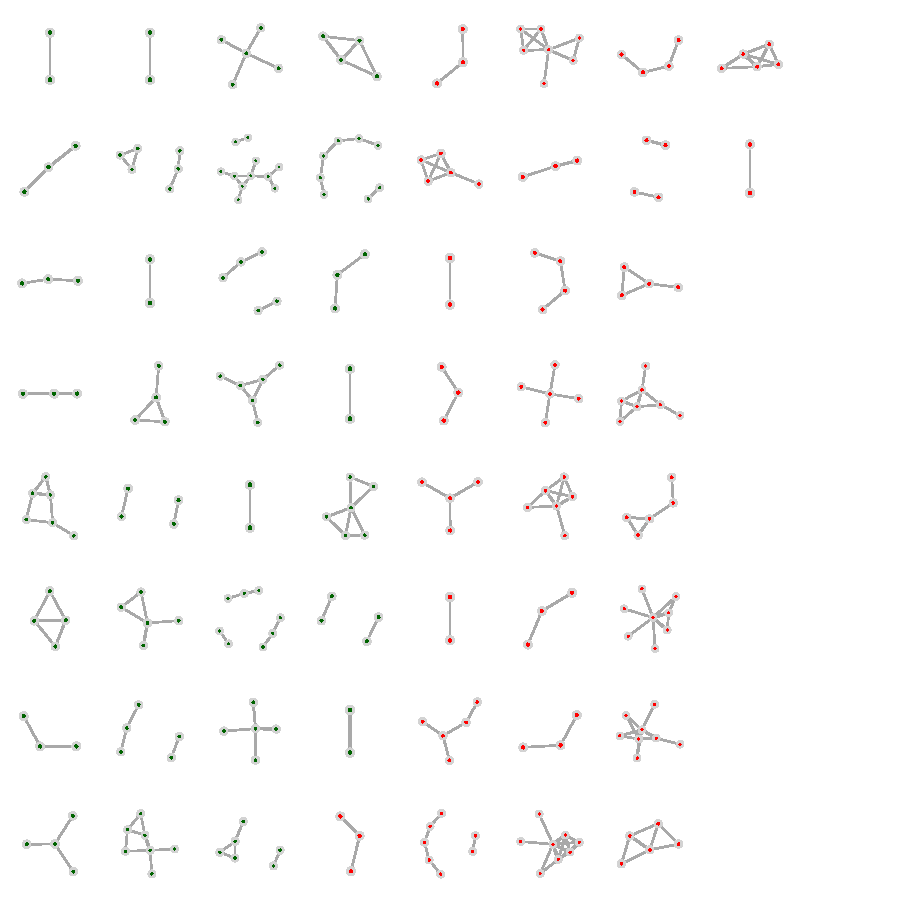
\includegraphics{notebook-002}

\begin{Schunk}
\begin{Sinput}
> ## Genotype average network 
> ## within each 
> liv.nets <- tree.nets[tree.info[,1] == 'live']
> sen.nets <- tree.nets[tree.info[,1] == 'sen']
> for (i in 1:length(liv.nets)){
+     diag(liv.nets[[i]]) <- 0
+     diag(sen.nets[[i]]) <- 0
+ }
> liv.cen <- unlist(lapply(liv.nets,function(x) centralization(x,FUN='degree')))
> sen.cen <- unlist(lapply(sen.nets,function(x) centralization(x,FUN='degree')))
> t.test(I(liv.cen-sen.cen))
\end{Sinput}
\begin{Soutput}
	One Sample t-test

data:  I(liv.cen - sen.cen)
t = -1.3324, df = 35, p-value = 0.1914
alternative hypothesis: true mean is not equal to 0
95 percent confidence interval:
 -0.22098995  0.04585768
sample estimates:
  mean of x 
-0.08756614 
\end{Soutput}
\begin{Sinput}
> 
\end{Sinput}
\end{Schunk}

Analyze the mean networks for live and senescent leaves.

\begin{Schunk}
\begin{Sinput}
> liv.mu <- meanNet(liv.nets)
> liv.var <- varNet(liv.nets)
> sen.mu <- meanNet(sen.nets)
> sen.var <- varNet(sen.nets)
> par(mfrow=c(1,2),mai=rep(0.1,4))
> gplot(liv.mu,gmode='graph',
+       edge.lwd=liv.mu/max(liv.mu)*3,vertex.col='green',
+       vertex.border='lightgrey',
+       edge.col=grey(liv.var/max(liv.var)),vertex.cex=2,
+       mode='circle',displaylabels=TRUE)
> gplot(sen.mu,gmode='graph',
+       edge.lwd=sen.mu/max(sen.mu)*3,vertex.col='red',
+       vertex.border='lightgrey',
+       edge.col=grey(sen.var/max(sen.var)),vertex.cex=2,
+       mode='circle',displaylabels=TRUE)
> 
\end{Sinput}
\end{Schunk}
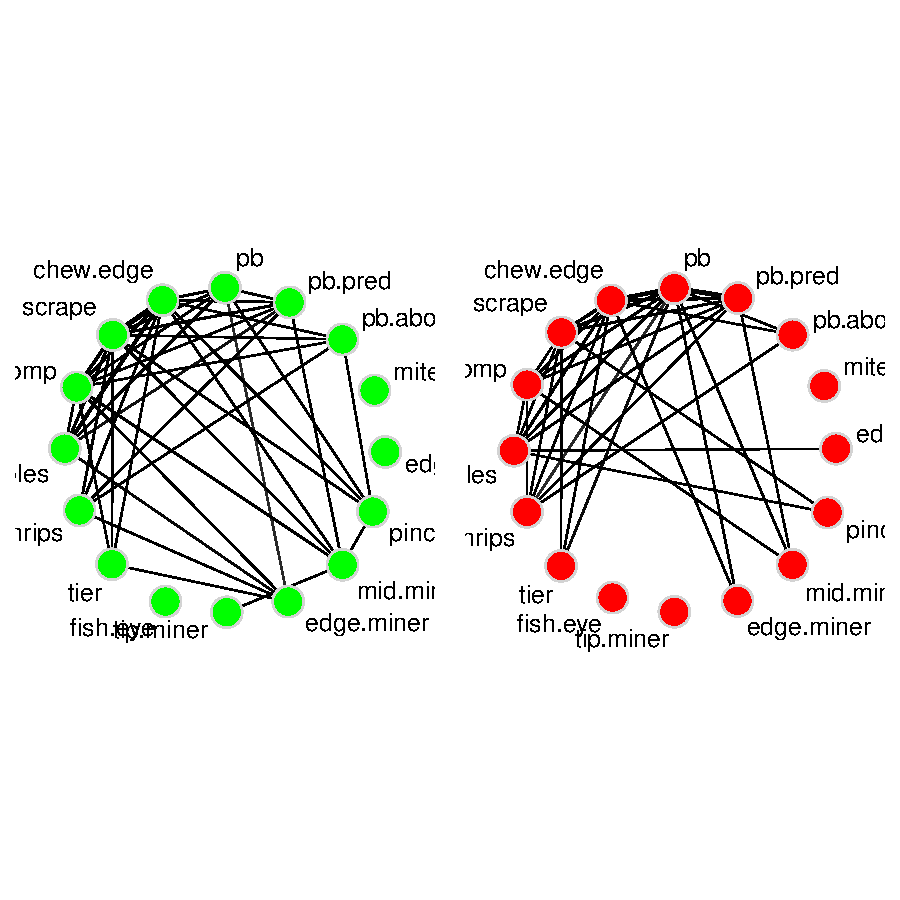
\includegraphics{notebook-004}

No relationship between the number of senescing leaves sampled and the difference in degree between networks.

\begin{Schunk}
\begin{Sinput}
> n.lfs <- tree.info$leaves[tree.info$leaf.type == 'sen']
> cor.test(n.lfs,I(liv.deg-sen.deg))
\end{Sinput}
\begin{Soutput}
	Pearson's product-moment correlation

data:  n.lfs and I(liv.deg - sen.deg)
t = -1.6598, df = 34, p-value = 0.1062
alternative hypothesis: true correlation is not equal to 0
95 percent confidence interval:
 -0.55260581  0.06017414
sample estimates:
       cor 
-0.2737739 
\end{Soutput}
\begin{Sinput}
> plot(I(liv.deg-sen.deg),n.lfs)
> 
\end{Sinput}
\end{Schunk}
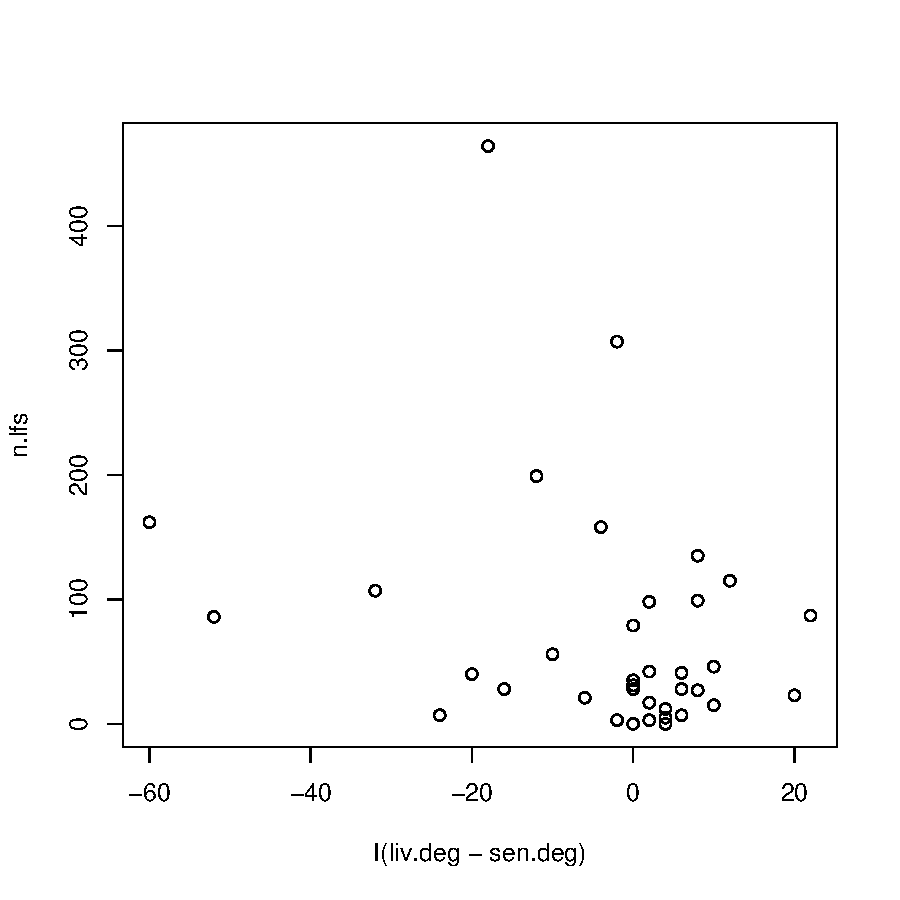
\includegraphics{notebook-005}

How much variance in network structure does genotype explain?

About 8\% of the variation in network structure was attributable to
tree genotype. This was primarily due to genetic effects on re-wiring of the network rather than changes to the structure. Leaf senescence strongly impacted network modularity. 

\begin{Schunk}
\begin{Sinput}
> library(BiodiversityR)
> dn.tree <- distNet(tree.nets)
> adonis(dn.tree~factor(leaf.type)*factor(geno),data=tree.info, strata=tree.info$tree)
\end{Sinput}
\begin{Soutput}
Call:
adonis(formula = dn.tree ~ factor(leaf.type) * factor(geno),      data = tree.info, strata = tree.info$tree) 

Blocks:  strata 
Permutation: free
Number of permutations: 999

Terms added sequentially (first to last)

                               Df SumsOfSqs MeanSqs F.Model      R2 Pr(>F)    
factor(leaf.type)               1    118.53 118.528  5.3315 0.07390  0.001 ***
factor(geno)                    7    123.52  17.646  0.7937 0.07702  0.005 ** 
factor(leaf.type):factor(geno)  7    116.79  16.684  0.7505 0.07282  0.626    
Residuals                      56   1244.97  22.232         0.77626           
Total                          71   1603.81                 1.00000           
---
Signif. codes:  0 ‘***’ 0.001 ‘**’ 0.01 ‘*’ 0.05 ‘.’ 0.1 ‘ ’ 1
\end{Soutput}
\begin{Sinput}
> ord.tree <- nmds.min(nmds(dn.tree,2,2),dims=2)
\end{Sinput}
\begin{Soutput}
Using random start configuration 
Using random start configuration 
Using random start configuration 
Using random start configuration 
Using random start configuration 
Using random start configuration 
Using random start configuration 
Using random start configuration 
Using random start configuration 
Using random start configuration 
Minimum stress for given dimensionality:  0.1615769 
r^2 for minimum stress configuration:  0.9430878 
\end{Soutput}
\begin{Sinput}
> spp.vectors <- envfit(ord.tree,spp.tot)
> spp.vectors <- envfit(ord.tree,spp.tot[,spp.vectors$vectors$pvals <= 0.05])
> plot(ord.tree,pch=19,
+      col=as.numeric(factor(tree.info$geno)))
> mu <- ch.plot(ord.tree,factor(tree.info$geno))
> points(mu,col=as.numeric(factor(unique(tree.info$geno))),pch=19,cex=1.5)
> plot(spp.vectors,col='darkgrey')
> legend('topright',legend=unique(tree.info$geno),col=as.numeric(factor(unique(tree.info$geno))),pch=19,bty='d',bg='white',box.col='lightgrey')
> 
\end{Sinput}
\end{Schunk}
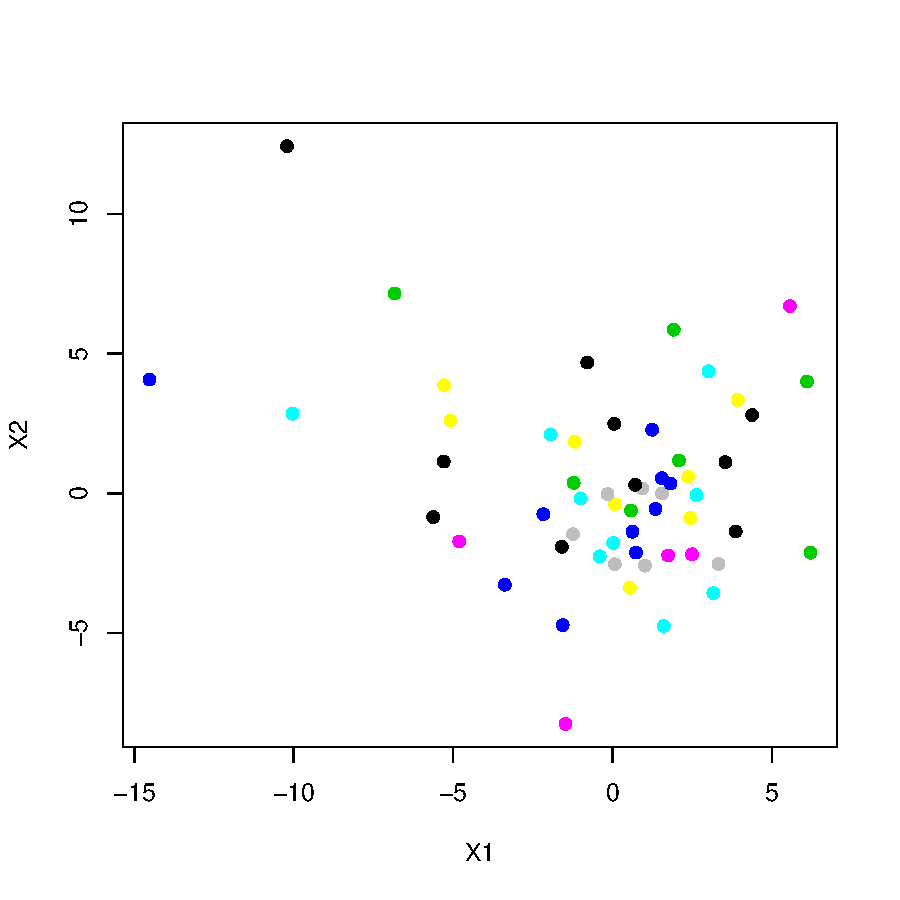
\includegraphics{notebook-006}

\begin{Schunk}
\begin{Sinput}
> library(bipartite)
> ### centrality
> tree.cen <- unlist(lapply(tree.nets,function(x) centralization(x,FUN='degree')))
> tree.mod <- dget(file='../data/tree.mod') # see src/treeMods.R
> summary(aov(tree.cen~tree+factor(leaf.type)*factor(geno),data=tree.info))
\end{Sinput}
\begin{Soutput}
                               Df Sum Sq Mean Sq F value Pr(>F)
tree                           35 2.9209 0.08345   1.311  0.232
factor(leaf.type)               1 0.1380 0.13802   2.168  0.152
factor(leaf.type):factor(geno)  7 0.6164 0.08805   1.383  0.251
Residuals                      28 1.7824 0.06366               
\end{Soutput}
\begin{Sinput}
> summary(aov(tree.mod~tree+factor(leaf.type)*factor(geno),data=tree.info))
\end{Sinput}
\begin{Soutput}
                               Df Sum Sq Mean Sq F value   Pr(>F)    
tree                           35 1.0698  0.0306   0.903 0.616910    
factor(leaf.type)               1 0.5749  0.5749  16.976 0.000304 ***
factor(leaf.type):factor(geno)  7 0.2974  0.0425   1.255 0.307767    
Residuals                      28 0.9482  0.0339                     
---
Signif. codes:  0 ‘***’ 0.001 ‘**’ 0.01 ‘*’ 0.05 ‘.’ 0.1 ‘ ’ 1
\end{Soutput}
\begin{Sinput}
> 
\end{Sinput}
\end{Schunk}

Genotype does not directly influence senescence, but may indirectly
influence senescence through pb.

\begin{Schunk}
\begin{Sinput}
> summary(aov(I(leaves^0.5)~factor(geno)*pb,
+             data=data.frame(tree.info,spp.tot)[tree.info$leaf.type == 'sen',]))
\end{Sinput}
\begin{Soutput}
                Df Sum Sq Mean Sq F value Pr(>F)  
factor(geno)     7  171.2   24.46   1.178 0.3564  
pb               1   98.8   98.82   4.760 0.0406 *
factor(geno):pb  6   79.5   13.25   0.638 0.6985  
Residuals       21  436.0   20.76                 
---
Signif. codes:  0 ‘***’ 0.001 ‘**’ 0.01 ‘*’ 0.05 ‘.’ 0.1 ‘ ’ 1
\end{Soutput}
\begin{Sinput}
> summary(aov(I(pb^0.5)  ~ factor(geno),
+             data=data.frame(tree.info,spp.tot)[tree.info$leaf.type == 'sen',]))
\end{Sinput}
\begin{Soutput}
             Df Sum Sq Mean Sq F value Pr(>F)  
factor(geno)  7  30.03   4.290   2.114 0.0751 .
Residuals    28  56.81   2.029                 
---
Signif. codes:  0 ‘***’ 0.001 ‘**’ 0.01 ‘*’ 0.05 ‘.’ 0.1 ‘ ’ 1
\end{Soutput}
\begin{Sinput}
> par(mfrow=c(1,2))
> plot(pb~geno,
+      data=data.frame(tree.info,spp.tot)[tree.info$leaf.type == 'sen',],
+      xlab='Genotype',ylab=expression(italic('P. betae')))
> plot(leaves~pb,
+      data=data.frame(tree.info,spp.tot)[tree.info$leaf.type == 'sen',],
+      xlab=expression(italic('P. betae')),ylab='Senescing Leaves Surveyed')
> abline(lm(leaves~pb,data=data.frame(tree.info,spp.tot)[tree.info$leaf.type == 'sen',]))
> 
\end{Sinput}
\end{Schunk}
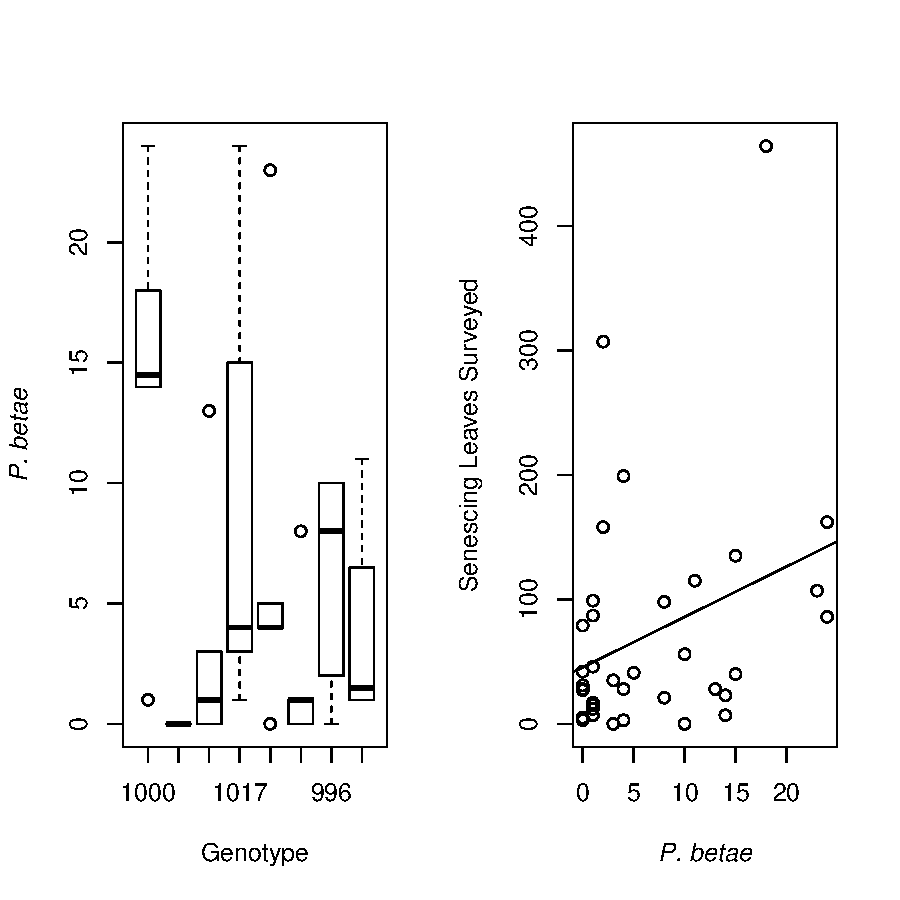
\includegraphics{notebook-008}

Stand level network modularity

\begin{Schunk}
\begin{Sinput}
> liv.bpn <- spp.tot[tree.info$leaf.type == 'live',]
> sen.bpn <- spp.tot[tree.info$leaf.type == 'sen',]
> liv.modules <- dget('../data/liv.modules')
> sen.modules <- dget('../data/sen.modules')
> par(mfrow=c(1,2))
> plotweb(liv.bpn);title(main='Live')
> plotweb(sen.bpn);title(main='Senescent')
> 
\end{Sinput}
\end{Schunk}
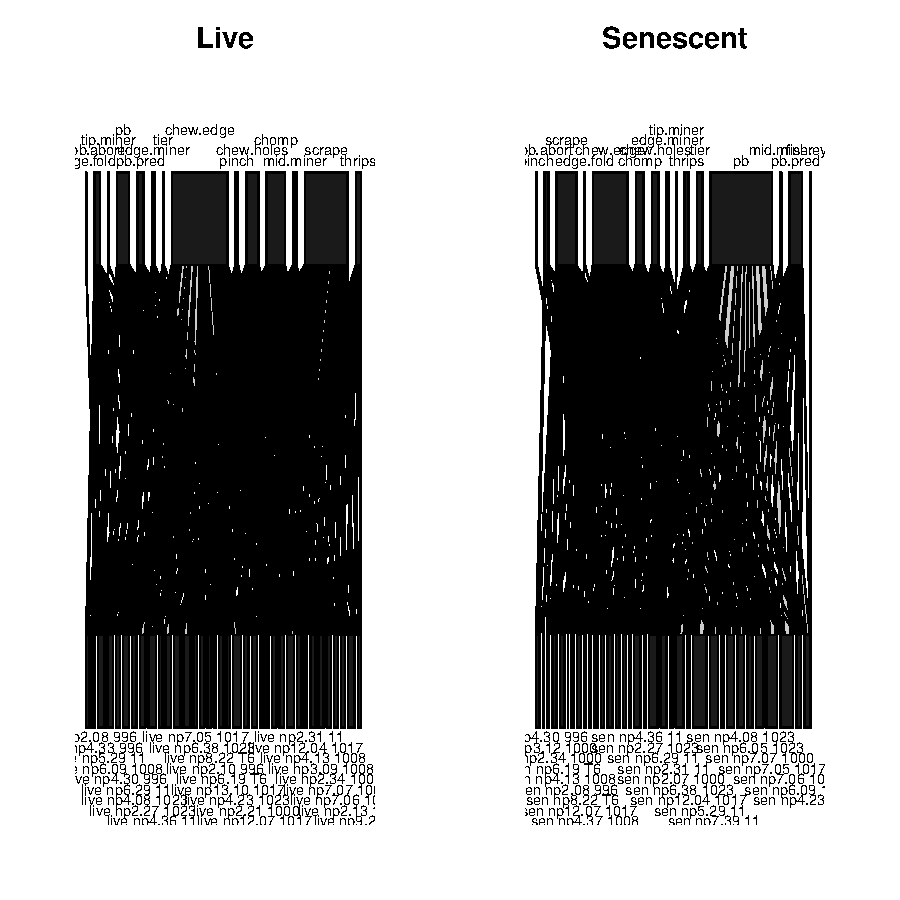
\includegraphics{notebook-009}

How does the mean interaction network compare to the bipartite to
unipartite projection?

\begin{Schunk}
\begin{Sinput}
> liv.b2u <- t(liv.bpn) %*% liv.bpn
> sen.b2u <- t(sen.bpn) %*% sen.bpn
> par(mfrow=c(2,2))
> liv.coo <- gplot(liv.mu,gmode='graph',displaylabels=TRUE)
> sen.coo <- gplot(sen.mu,gmode='graph',displaylabels=TRUE)
> gplot(liv.b2u,coord=liv.coo,gmode='graph',displaylabels=TRUE)
> gplot(sen.b2u,coord=sen.coo,gmode='graph',displaylabels=TRUE)
> 
\end{Sinput}
\end{Schunk}
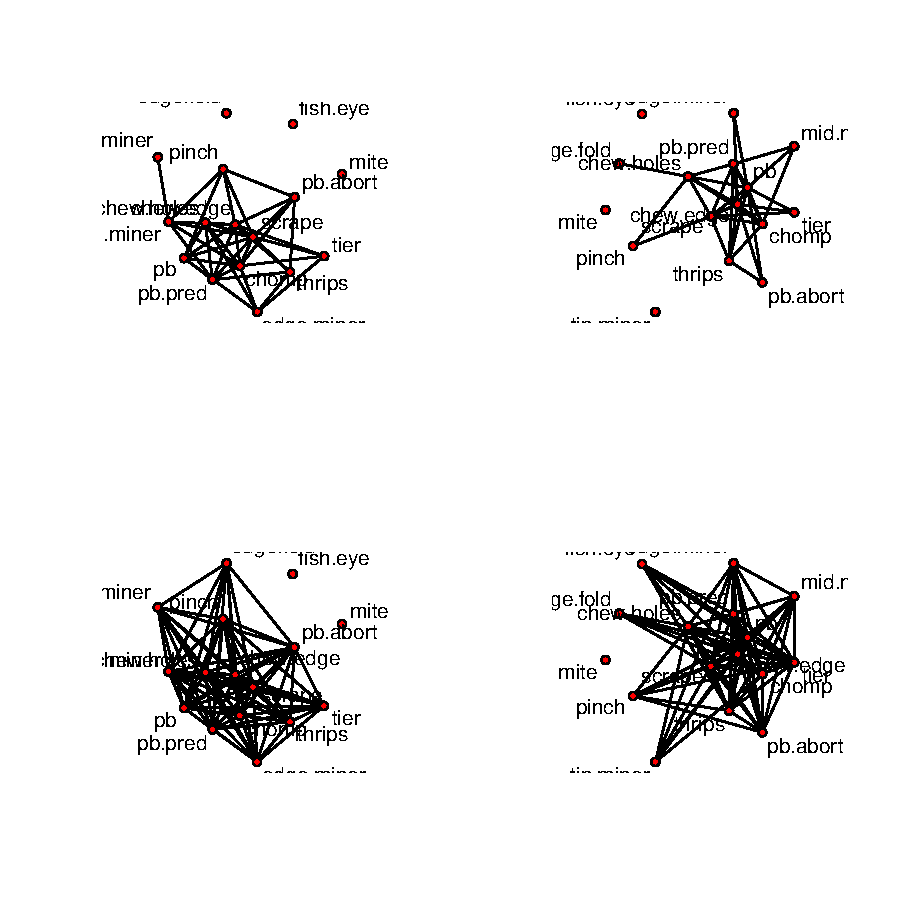
\includegraphics{notebook-010}

\section{12 Mar 2014}

Summary of analyses below:

\begin{enumerate}
\item Genotype does not affect SES
\item Genotype affects multivariate co-occurrence patterns for live
  (negative co-occurrences) and senescent (positive co-occurrences)
  leaves. These data are relatvized to co-occurrence maximum and use
  the Clarke adjustment.
\end{enumerate}

\begin{Schunk}
\begin{Sinput}
> library(vegan)
> pit <- read.csv('~/projects/dissertation/projects/acn/data/arth_cooc_PIT_Lau.csv')
>                                         #
> coMat = function(x,type=c('pos','neg')){
+   if (length(type)!=1|all(type!=c('pos','neg'))){print('Using positive co-occurrence');type='pos'}
+   if (length(colnames(x))==0){colnames(x) <- paste('sp',1:ncol(x),sep='')}
+   if (type=='neg'){print('Using negative co-occurrence')}
+   x <- sign(x)
+   y <- list()
+   k <- 0
+   for (i in 1:ncol(x)){
+     for (j in i:ncol(x)){
+       k <- k+1
+       if (i!=j){
+         if (type=='pos'){
+           y[[k]] <- (x[,i]+x[,j])
+           y[[k]][y[[k]]!=2] <- 0
+           y[[k]] <- sign(y[[k]])
+         }else{
+           y[[k]] <- (x[,i]+x[,j])
+           y[[k]][y[[k]]!=1] <- 0
+           y[[k]] <- sign(y[[k]])
+         }
+         names(y)[k]=paste(colnames(x)[i],colnames(x)[j],sep='_')
+       }
+     }
+   }
+   y=do.call(cbind,y)
+   return(y)
+ }
>                                         #got through each tree and quantify the number of co-occurrences for all species pairs
>                                         #get pit info
> pit.env <- pit[,1:6]
>                                         #no fungal
> pit.com <- pit[,-1:-7]
> pit.com[is.na(pit.com)] <- 0
>                                         #combine pb.upper and pb.lower and woody
> pit.com[,4] <- pit.com[,4] + pit.com[,6] + pit.com[,8]
> colnames(pit.com)[4] <- 'pb'
> pit.com <- pit.com[,c(-6,-8)]
>                                         #combine pb. preds
> pit.com[,5] <- pit.com[,5] + pit.com[,7] 
> pit.com <- pit.com[,-7]
>                                         #remove pb holes and mite
> pit.com <- pit.com[,c(-6,-17)]
> ###Separate into trees
> pit.com <- split(pit.com,paste(pit.env$tree,pit.env$leaf.type))
> pit.g <- unlist(lapply(split(pit.env$geno,paste(pit.env$tree,pit.env$leaf.type)),function(x) as.character(x[1])))
> pit.lf <- unlist(lapply(split(pit.env$leaf.type,paste(pit.env$tree,pit.env$leaf.type)),function(x) as.character(x[1])))
> pit.cooc <- lapply(pit.com,coMat,type='neg')
> pit.cooc <- lapply(pit.cooc,function(x) apply(x,2,sum))
> pit.cooc <- do.call(rbind,pit.cooc)
> pit.neg <- pit.cooc
> pit.cooc <- lapply(pit.com,coMat,type='pos')
> pit.cooc <- lapply(pit.cooc,function(x) apply(x,2,sum))
> pit.cooc <- do.call(rbind,pit.cooc)
> pit.pos <- pit.cooc
> pit.com. <- do.call(rbind,lapply(pit.com,function(x) apply(x,2,sum)))
>                                         #
> adonis(apply(pit.com.,2,function(x) if (all(x==0)){x}else{x/max(x)})[pit.lf=='live',]~pit.g[pit.lf=='live'])
> adonis(apply(pit.com.,2,function(x) if (all(x==0)){x}else{x/max(x)})[pit.lf=='sen',]~pit.g[pit.lf=='sen'])
>                                         #
> adonis(cbind(pit.cooc[pit.lf=='live',],ds=rep(1,nrow(pit.cooc[pit.lf=='live',])))~pit.g[pit.lf=='live'],perm=5000)
> adonis(cbind(pit.cooc[pit.lf=='sen',],ds=rep(1,nrow(pit.cooc[pit.lf=='sen',])))~pit.g[pit.lf=='sen'],perm=5000)
> adonis(cbind(apply(pit.cooc[pit.lf=='live',],2,function(x) if (all(x==0)){x}else{x/max(x)}),ds=rep(0.1,nrow(pit.cooc[pit.lf=='live',])))~pit.g[pit.lf=='live'],perm=5000)
> adonis(cbind(apply(pit.cooc[pit.lf=='sen',],2,function(x) if (all(x==0)){x}else{x/max(x)}),ds=rep(0.1,nrow(pit.cooc[pit.lf=='sen',])))~pit.g[pit.lf=='sen'],perm=5000)
>                                         #
> barplot(sort(apply(pit.cooc[pit.lf=='live',],2,sum),dec=TRUE)[1:10],las=2)
> barplot(sort(apply(pit.cooc[pit.lf=='sen',],2,sum),dec=TRUE)[1:10],las=2)
>                                         #ses
> source('~/projects/packages/cooc/src/cooc.R')
> pit.ses. <- lapply(pit.com,function(x) if (length(table(x))<2){NA}else{oecosimu(x,cs,method='r1',burnin=100,thin=10,nsimul=1000)$oecosimu})
> pit.ses <- unlist(lapply(pit.ses.,function(x) unlist(x[1])))
> pit.ses.p <- unlist(lapply(pit.ses.,function(x) unlist(x[3])))
> pit.ses[is.na(pit.ses)] <- 0
> summary(aov(pit.ses[pit.lf=='live']~pit.g[pit.lf=='live']))
> summary(aov(pit.ses[pit.lf=='sen']~pit.g[pit.lf=='sen']))
> pit.ses[pit.lf=='live']~pit.g[pit.lf=='live']
>                                         #reml for ses
> source('/Users/Aeolus/projects/packages/ComGenR_development/src/cgREML.R')
> cgREML(pit.ses[pit.lf=='live'],pit.g[pit.lf=='live'])
> cgREML(pit.ses[pit.lf=='sen'],pit.g[pit.lf=='sen'])
> cgREML((pit.ses[pit.lf=='sen']-pit.ses[pit.lf=='live']),pit.g[pit.lf=='sen'])
> 
\end{Sinput}
\end{Schunk}

\section{3 Feb 2014}

Figures

\begin{Schunk}
\begin{Sinput}
> library(gplots)
>                                         #PB among genotypes
> mu <- tapply(pbp[type.t=='live']*100,geno.t[type.t=='live'],mean)
> se <- tapply(pbp[type.t=='live']*100,geno.t[type.t=='live'],function(x) sd(x)/sqrt(length(x)))
> se <- se[order(mu,decreasing=TRUE)]
> mu <- mu[order(mu,decreasing=TRUE)]
> barplot2(mu,plot.ci=TRUE,ci.u=mu+se,ci.l=mu-se,ylab='P. betae abundance (percent leaves)',xlab='Tree Genotype',ylim=c(0,20))
>                                         #Composition among genotypes for living leaves
> nms.liv <- nmds.min(nmds(vegdist(com.i[type.t=='live',])))
> ch.plot(nms.liv,g=geno.t[type.t=='live'])
> pb.env <- data.frame('P_betae'=pbp[type.t=='live'])
> pbp.fit <- envfit(nms.liv,pb.env)
> plot(pbp.fit,col='darkgrey')
>                                         #co-occurrence network plots
> 
> net.t <- lapply(split(pit.com,type),CoNetwork)
> for (i in 1:length(net.t)){
+   rownames(net.t[[i]]) <- colnames(net.t[[i]]) <- paste('S',1:ncol(net.t[[i]]),sep='')
+ }
> coord <- mgp(net.t[[1]],split(pit.com,type)[[1]],displaylabels=TRUE)
> par(mfrow=c(1,1))
> mgp(net.t[[1]],split(pit.com,type)[[1]],loc=FALSE,my.coord=coord,displaylabels=TRUE)
> mgp(net.t[[2]],split(pit.com,type)[[2]],loc=FALSE,my.coord=coord,displaylabels=TRUE)
>                                         #barplot of p betae 1,2,3,4 gall leaves
> 
> 
> stopme
> 
> 
\end{Sinput}
\end{Schunk}


\section{30 Jan 2014}

Continuing to work on script.

Results Summary

\begin{itemize}
\item Richness
  \begin{itemize}
  \item Genotype does not influence richness (Live: 1.4102840
    0.2350093 , Sen: 1.060422 0.303119 )
  \item Or the difference in richness (-2.246907e-09  1.000000e+00)
  \end{itemize}
\item Composition
  \begin{itemize}
  \item Leaf type influences composition (Paired t: t = 23.7363, df = 34, p-value < 2.2e-16)
  \item Genotype does not influence the difference in community
    composition between leaf types (REML: chi2=0.53,P=0.465)
  \item Genotype influences community composition for live but not sen
    leaves (F=1.85,P=0.004,R2=0.28; F=1.22,P=0.176)
  \item Several genotypes are different (Paired Perm: 1000 vs
    T6,1008vs1023vsT6, 1023vs11vsT6, 11vs996,996vsT6)
  \end{itemize}
\item PB effects: 
  \begin{itemize}
  \item PB (as percent) decreased from senescent to live leaves by 31\% on average
    (t = -5.5791, df = 34, p-value = 3.036e-06) but this was not
    different among genotypes (X2=2.809,P=0.0937)
  \item PB.total ~ Genotype (X2=4.20104879,P=0.0404) 
  \item Percent PB ~ Genotype Live (X2=6.75,P=0.009), Percent PB !~ Genotype Sen (X2=3.32,P=0.07)
  \item PB frequencies are different among genotypes (X2 test: 125.62,
    df=18, P=2.2e-16), frequencies of 0 and 1 PB per leaf are
    different among genotypes on live leaves (X2=6.701,P=0.0096 and
    X2=6.27,P=0.012), while 2 PB/leaf for SEN (X2=4.045,P=0.044)
  \end{itemize}
\item These species' abundances differ between live and senescent:
  \begin{itemize}
  \item chew.edge (P=0.00009)
  \item scrape (P=0.000)
  \item chomp (P=0.00013)
  \item chew.holes (P=0.00553)
  \item tier (P=0.01134)
  \item mid.miner (P=0.00553)
  \item pinch (P=0.00683)
  \item pb (P=0.00060)
  \end{itemize}
\item Co-occurrence patterns
  \begin{itemize}
  \item Live SES is lower than sen ses (Live: SES=-7.865,P=0.001; Sen: SES=-4.447,P=0.001)
  \item No genotype effect on co-occurrence patterns within trees (X2=0,P=1)
  \item Co-occurrence network structure different between live and sen
    (QAP: z=7.454,P<0.0001).
  \end{itemize}
\item Nestedness
  \item At the tree scale, both live and sen are nested for r00 and r0
  \item At the genotype scale, live is nested for r00 and both for r0
\end{itemize}

\section{29 Jan 2014}

Analyze data for the following:

- Genetic effect on P. betae \\
- Genetic effect on composition \\
- Genetic effect on SES \\
- Co-occurrence network structure \\
- Nestedness for live and senesced \\


\section{4 Dec 2013}
Notes from meeting with Tom:

\begin{itemize}
\item P. betae phenology likely done by late June (see Williams and Whitham)
\item Test for number of senescing leaves correlation with Pb
\item Think about direct versus indirect genetic effects on community
\item Test genotype effect on all species
\item Get genetic distance data (RFLP?), maybe ask Zaccheus
\item Think about genetic basis of leaf abscision/senescence
\end{itemize}

\section{2 Dec 2013}

Results of analysis of liv and sen
\begin{itemize}
\item Networks are sparse but show distinct differences, need to
  figure out how to compare models
\item Co-occurrence
%%%Arthropods only

%%%Arthropods and Fungi
\item Co-occurrence increases after senescence (t = 2.1951, df = 30, p-value = 0.03603)
\item Genotype effect live: geno.ses     6  22.46   3.743   1.006  0.441
\item Genotype effect sen: geno.ses     6  33.59   5.599   4.699
  0.002 **geno.ses     6  33.59   5.599   4.699  0.002 **
\item Genotype mean ses shift from some positive to all negative going
  from sen to liv

\item Greater percent pemphigus on sen than live (t = 5.4687, df = 34, p-value = 4.226e-06)
\item No difference in fungus (t = -1.8687, df = 34, p-value = 0.07031)
\end{itemize}

\textbf{Dataset Alterations}
\begin{enumerate}
\item Check the following
  \begin{enumerate}
  \item np5.5 doesn't exist but "NP6-5  1023       1   M"
  \item np13.10 1017_live - "235 NP13-10  1017       1   M"
  \item np2.4 1023_live - "199 NP2-4 1000C       0   F"
  \item "np3.36 1000_live"  "np3.36 11_sen" - "168 NP3-36  1000       0   F"
  \item np4.23 1023_sen - "147 NP4-23  1023       1   M"
  \end{enumerate}
\item np5.5 does not exist in the pit dataset, changing to np6.5
\item np3.36 is genotype 1000, changing in dataset from 11 to 1000 for sen
\item np2.4 is 1000, but there is no np2.4 in the senescing dataset,
  make np2.4 into np4.23.
\item np13.10 missing in senescing dataset, make np13.10 sen zero.
\item All passed the following test:
\begin{verbatim}
    all(sort(unique(paste(test[[1]]$geno,test[[1]]$tree)))==sort(unique(paste(test[[2]]$geno,test[[2]]$tree))))
\end{verbatim}
\end{enumerate}

Notes from samples:

\begin{itemize}
\item NP2-10 996 tree: almost all leaves from one branch, which
  appeared to be dying back.
\item NP8.22 T6 tree: "weird"
\item NP6.05 1023 tree: check tree number. Could be NP5.05.
\item np2.21 1000 tree: pair of green leaves with galls and leaf tier
\item np4.23 1023 tree: should it be np4.27?
\item np5.25 996 tree: yellow leaf with gall tied to one green leaf
  (no gall), which fell apart
\item np3.12 1000 tree: fungal branch infection on most branches. Most
  leaves from 3 branches
\item np3.36 11 tree: 1000? check litter and garden info
\end{itemize}

\section{26 Nov 2013}



\section{15 Nov 2013}
\begin{itemize}
\item Wait to process litter leaves, they are mixed with other leaves
  and would need to be sorted
\item Moving them into Bio340
\item Transporting senescing leaves back to Cambridge
\end{itemize}

\section{11 Nov 2013}

\begin{itemize}
\item Group woodies with non-woody
\item How do you handle the absence of senescent leaves?
\item What about the affect of Pemphigus loads on individual leaves or
  on trees?
\end{itemize}

\textbf{Senescent Leaf Data Collection Notes}

\begin{itemize}
\item Double check and correct np3.36 genotype from Master Sheet
\item Pb.upper = gall opening is on the upper side of the leaf
\item Fungal = necrotic tissue
\item Think about fungal from previous observations, maybe just call
  it necrosis
\end{itemize}

\section{7 Nov 2013}

\begin{itemize}
\item Running genotype sensitivity analysis
\item Not significantly different when removing just one genotype
\item Try removing more genotypes
\end{itemize}

\section{6 Nov 2013}

\begin{enumerate}
\item Decide on species groups 
\item Re-run analyses
\item Collect senescing and leaf litter data
\item Identify to species using Randy's notebook
\item Look into Gina's time paper
\item Serphid and Chanamyid flies

\end{enumerate}

\section{5 Nov 2013}

Running preliminary analyses.
\begin{enumerate}
\item Stand level networks (structure)
\item Tree level co-occurrence patterns (significant genotype effect)
\end{enumerate}


\section{Before 15 Oct 2013}

\subsection{Tasks}
\begin{itemize}
\item Photograph representatives of all leaf mods
\item Measure average specific leaf area for each shoot
\item Weigh leaf mods where possible
\item Run co-occurrence analyses on leaf modifiers
\item Run analysis of genotypic effect on leaf mod co-occurrence
  patterns
\item Add covariates to genetic model
\end{itemize}


\textbf{Process Summary}
\begin{itemize}
\item ONC Co-Occurrence 2012
  \subitem Did a preliminary analysis of the co-occurrence data with
  tree level co-occurrence patterns among genotypes
  \subitem Significant genotype pattern of observed C-scores
  \subitem Average dp networks "look" different
  \subitem Can still average among shoots prior to analysis
  \subitem Need to check effects of the number of leaves sampled
\item Art's 2004-2006 data
\item Gina's 2002-2003 data
\end{itemize}


\textbf{Summary}

\begin{itemize}
\item Study the cooccurrence patterns of leaf modifying arthropods on
  different genotypes of Narrowleaf Cottonwood (\texit{Populus angustifolia}).

\end{itemize}

\subsection{Meta-data}
\begin{itemize}
\item Leaves collected from trees of known genotype in the north
  garden of the Ogden Nature Center on 4 May 2012.
\item Between 3 and 4 branches were cut from 15-20 feet on the west
  aspect of trees.
\item Branches were stored in water until the leaf shoots were removed
  from each branch.
\item Branches were between 0.5 and 1 cm in diameter
\item Small (~0.25 cm) green leafhoppers abundant
\item Leaves were stored in ziplock bags until processed (~ 1 week)
\item Leaf modifiers were scored at the leaf scale, keeping track of the
  identity of each shoot
\item Small, young/juvenile leaves close to the apical meristem were
  not surveyed, as they would not have equal exposure time to
  arthropods
\item NOTE: N4.30 P. betae tends to be higher up on the leaf above the
  junction of the leaf and the petiole
\item NOTE: In future studies, you can write the shoot number on the
  leaves, and possibly the leaf number
\item NOTE: Specimen N2-9 had many instances of some kind of black rot
  in the petioles that almost always coincided with pemphigus galls
  and sometime phylocolpa. It also occurred in petioles of adjacent
  stems without pemphigus when there was a high enough load. It seemed
  to grow both out of the gall and up from the stem into the
  petiole. Possibly an effect of nutrient dynamics? 
\end{itemize}


\subsection{PIT Tree Level Co-occurrence Data Aug 2012}

\subsection{Methods}
\begin{enumerate}
\item 20 shoots collected from between 2 and 3 meters height
\item leaves were collected haphazardly from around the entire tree
\item shaded leaves were avoided
\item abscising leaves were avoided
\item 5 leaves per shoot (n=10) for each tree starting from the bottom of the whorl at the first full sized leaf
%%%%%%%%%%%%%%%%%%%%%%%%%%%%%%%%%%%%%%%%%%%%%%%%
%%%%%%%%Leaf Modifier Descriptions
%%%%%%%%%%%%%%%%%%%%%%%%%%%%%%%%%%%%%%%%%%
\item The following leaf modifiers were assessed:
  \begin{itemize}
  \item p.upper (number): Pemphigus opening on upper side of leaf
  \item p.lower (number): Pemphigus opening on lower side
  \item p.nec (number): Pemphigus with necrosis
  \item p.hole (number): Pemphigus with chow hole
  \item p.woody (number): woody Pemphigus gall (likely a different
    species, check senescent leaves for opening location)
  \item p.open (number): Pemphigus that has been opened
  \item chew.edge (presence): chewing at the edge
  \item chew.holes (presence): chewing holes not at edge
  \item lace (presence): lacey chewing
  \item fish.eye (presence): hole with necrosis surrounding
  \item tip.miner (presence): mining at the tip
  \item edge.miner (presence): mining at the edge
  \item fungal (presence): fungal necrosis
  \item chomp (presence): large removal of tissue
  \item pinch (presence): pinching at the edge of the leaf
  \item thirps (presence): thrip damage (golden-brown hue with exuvia and frass)
  \end{itemize}
\end{enumerate}



%% %%Activate for bibtex vibliography
%% \cite{goossens93}
%% \bibliographystyle{plain}
%% \bibliography{/Users/Aeolus/Documents/bibtex/biblib}


\end{document}  


